\chapter{Magnetické vázání}

Velmi důležitým jevem, který jsme při dalším experimentování objevili, je, že dva spinnery umístěné blízko sebe, z nichž jeden je poháněn motorem\footnote{Tento spinner nazveme hnacím.}, se mohou magneticky vázat - tzn. že si hnaný a hnací spinner udržují nějaký konstantní poměr rychlostí.
Tomu, v jakém poměru jsou, budeme říkat "mód". Například, když jsou rychlosti hnaného a hnacího spinneru stejné, řekneme, že jsou v módu 1 ku 1 (značeno $1:1$). Později v této kapitole budeme tyto módy dále zkoumat a budeme vždy prvním číslem označovat rychlost hnaného spinneru a druhým číslem rychlost hnacího spinneru. Tento jev je obzvlášť důležitý, jelikož umožňuje tvorbu prvního primitivního druhu magnetického převodu.

\section{Měření magnetickým čidlem}

\begin{wrapfigure}{r}{0.5\textwidth}
    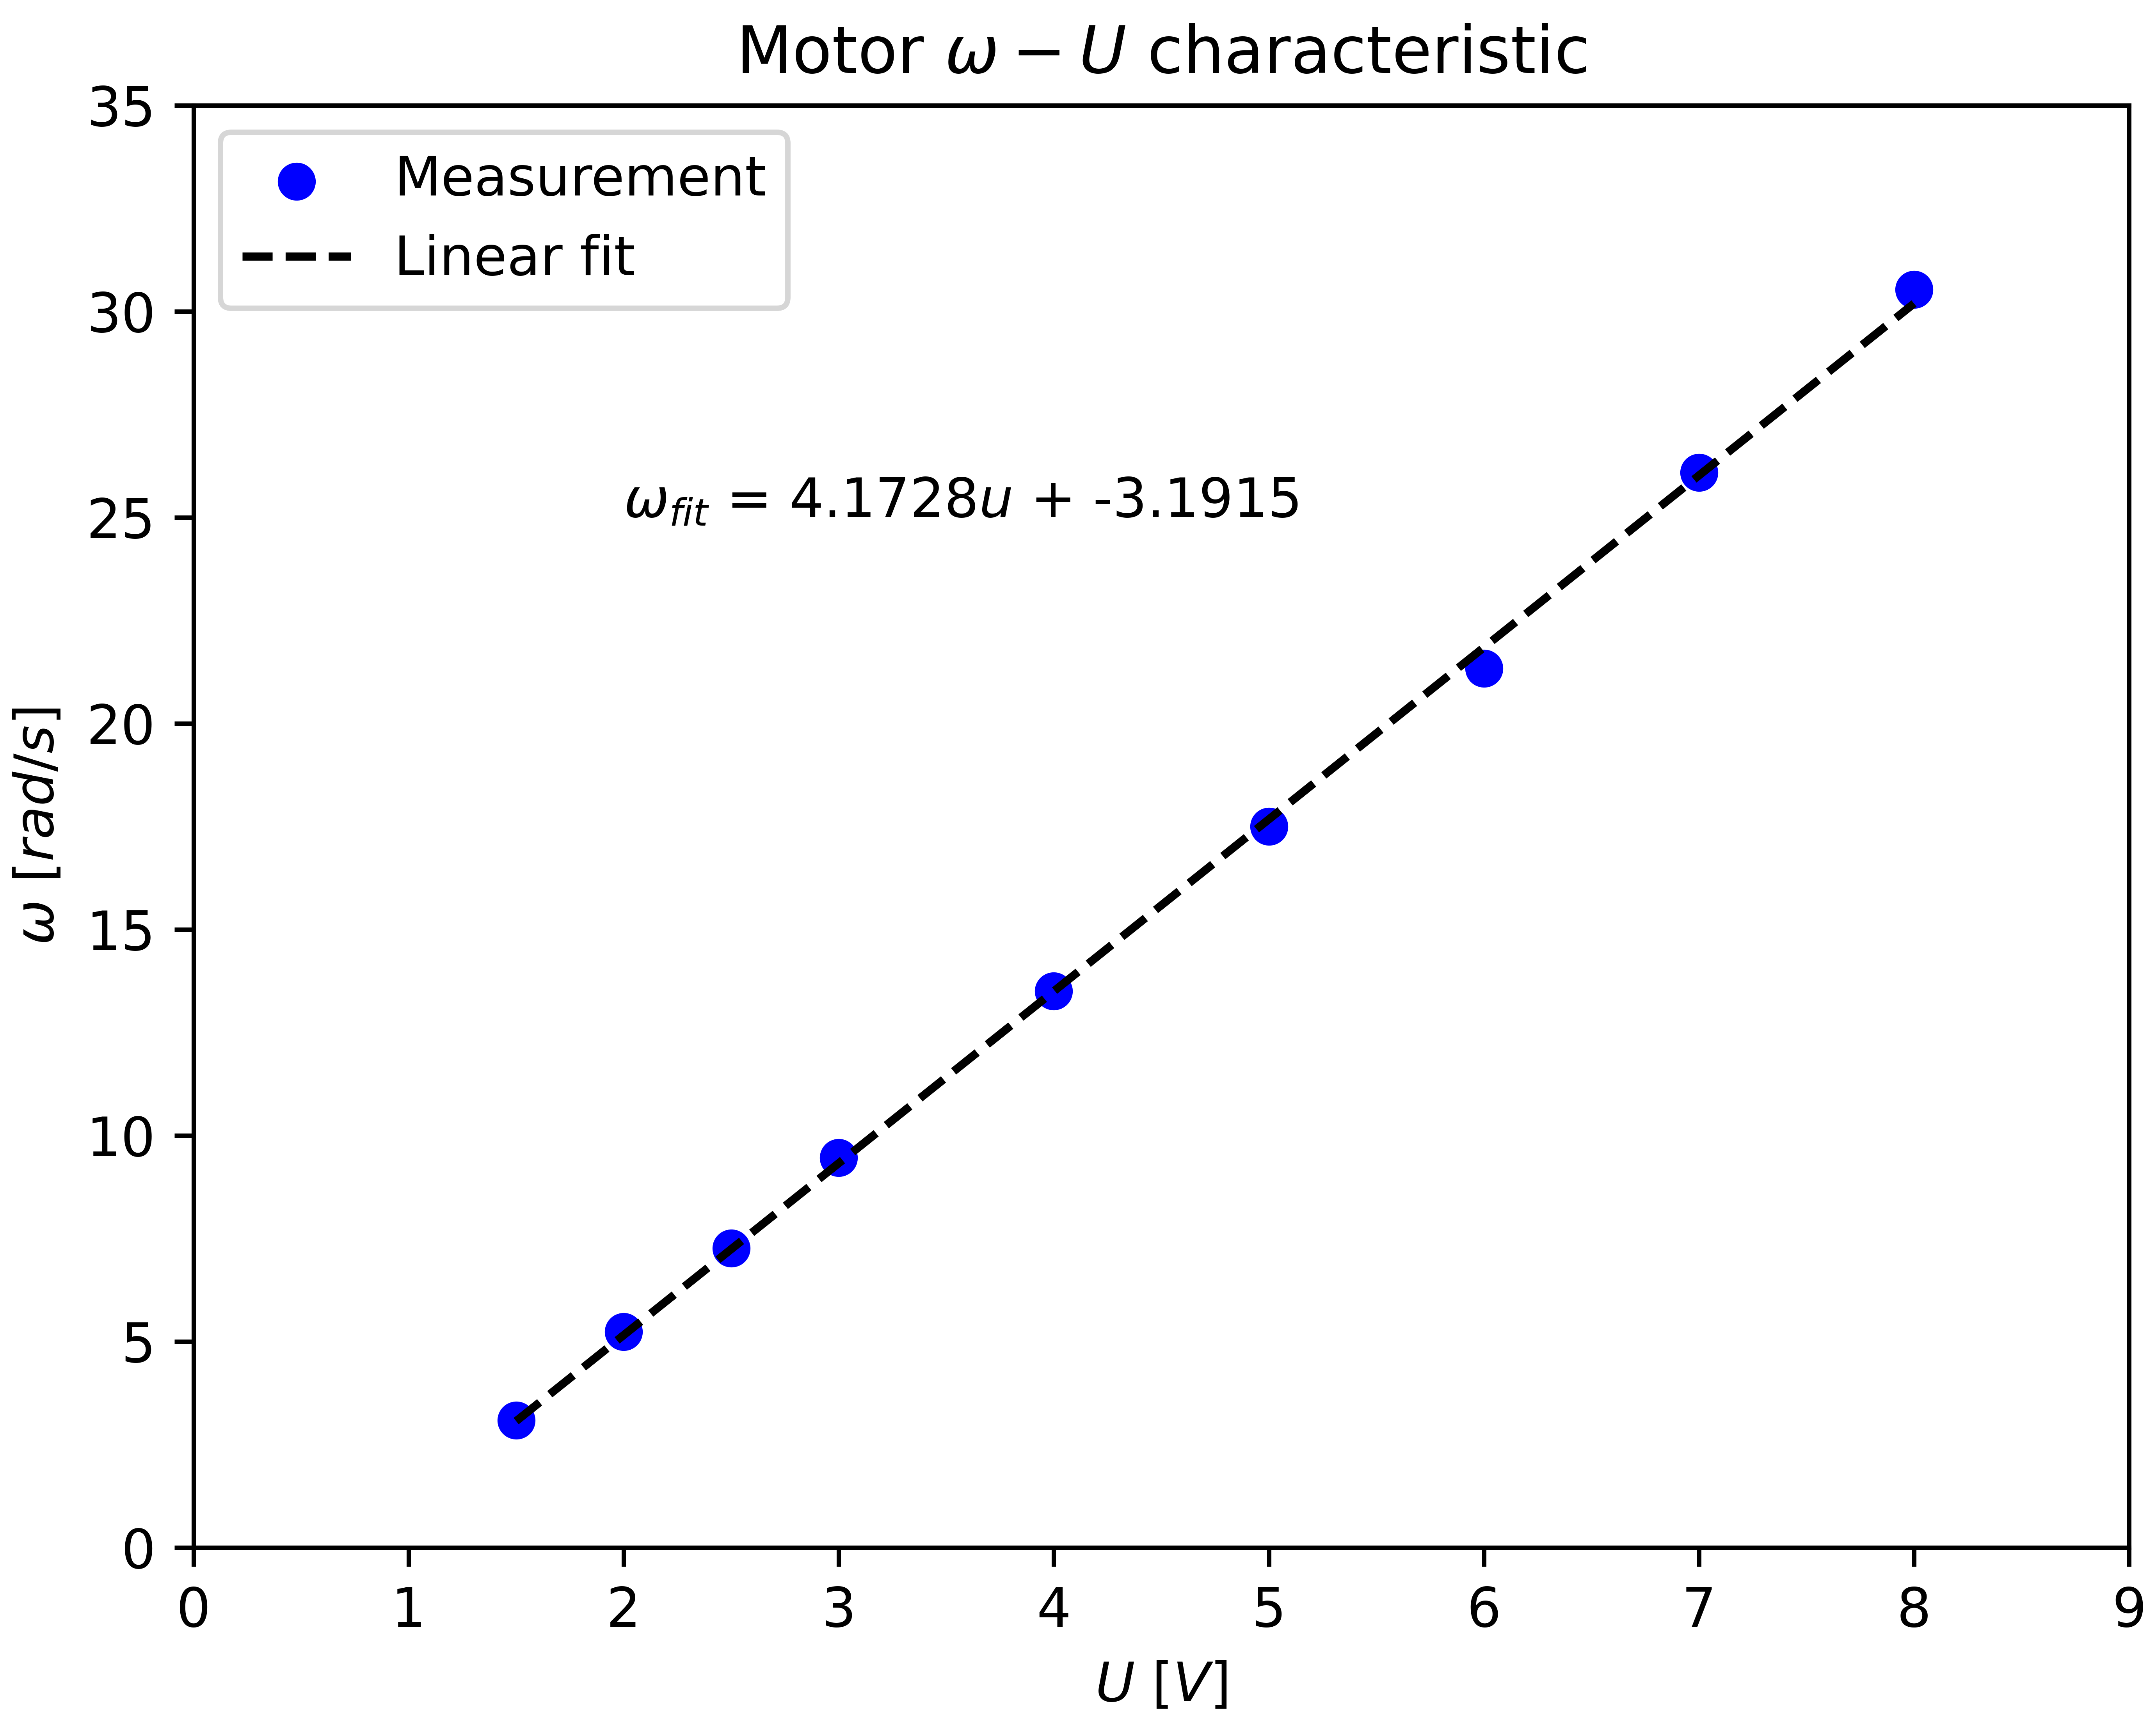
\includegraphics[width=0.42\textwidth]{motor_characteristic.png}
    \centering
    \caption[$\omega - U$ charakteristika motoru]{$\omega - U$ charakteristika motoru}
    \label{fig:motor_characteristic}
\end{wrapfigure}

Prvním způsobem, jak jsme se pokoušeli o sledování vázání spinnerů, bylo pomocí magnetického čidla Vernier, stejně jako na \autoref{fig:spinner_drag_aparature}. Rotaci hnaného spinneru jsme sledovali tímto čidlem, zatímco hnací spinner byl poháněn vrtačkou regulovanou laboratorním zdrojem napětí. Hnaný i hnací spinner byly pevně připevněny ve vzdálenosti 8cm (vzdálenost jejich středů).
Z hustoty naměřených peaků jsme opět určili přibližnou úhlovou rychlost hnaného spinneru (stejně jako v kódu \ref{code:4}). Rychlost hnacího spinneru jsme určili z napětí, kterým byla vrtačka poháněna, jelikož jsme pro ni dříve určili charakteristiku výstupní úhlové rychlosti v závislosti na napětí (viz \autoref{fig:motor_characteristic}).

Jak již bylo zmíněno, nevýhodou této metody je, že měření magnetickou sondou je velmi nepřesné a není schopné určit okamžitou rychlost. Další nevýhodou je, že magnetickou sondu jsme měli k dispozici pouze jednu. Přesto jsme byli schopni několik módů naměřit a porovnat se simulací a tyto výsledky jsou shrnuty v grafu \ref{fig:mag_coupling_vernier}.

\begin{figure}[!ht]
    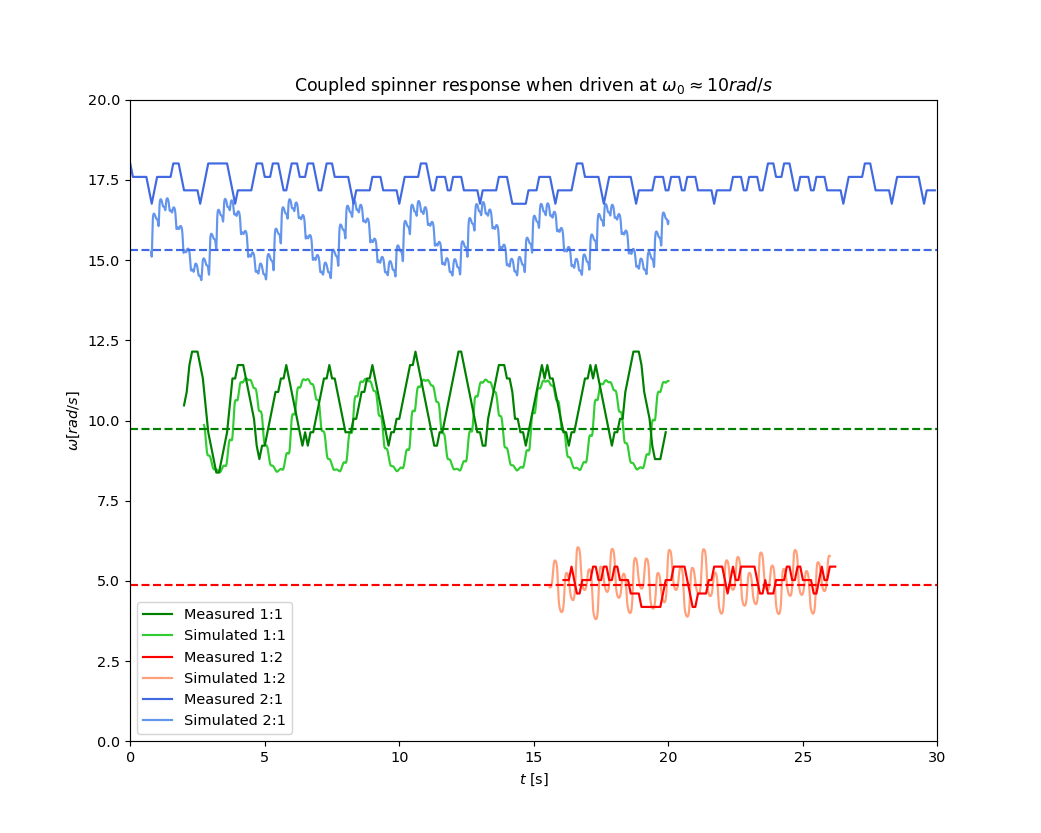
\includegraphics[width=\textwidth]{simulated_coupling.png}
    \centering
    \caption{Výsledky měření vázání prováděného magnetickým čidlem}
    \label{fig:mag_coupling_vernier}
\end{figure}

\section{Hlubší analýza}

Neuspokojivá přesnost výsledků získaných předchozí analýzou dat z magnetického čidla vedla k pokusům o vynalezení rozdílného způsobu zpracování dat, který by nám umožnil sledovat rychlost v průběhu jedné otáčky. Doposud nebylo možné tento detail získat, jelikož předchozí způsob pouze počítá jednotlivá otočení, ale ignoruje, jak jedna samotná otočka vypadá.

Nový způsob zpracování by měl stále být schopen analyzovat již naměřená data, abychom nemuseli měnit aparaturu ani měření provádět znovu. Nakonec jsme se rozhodli sledovat deformaci jednotlivých peaků průběhu magnetické indukce a z této deformace se snažit odhadnout a vyvodit přesný úhel spinneru v daném momentu. Do hloubky je tento proces popsán v další kapitole.

\clearpage
\subsection{Popis nového algoritmu}

Tento algoritmus je založen na tom, že nám bude známá závislost magnetického pole na úhlu spinneru. Pokud tuto závislost budeme znát a budeme mít nějaký nový záznam průběhu magnetické indukce v čase, jsme schopni zpětně vyvodit, jaký musel být průběh úhlu v čase.

Celý proces tedy začíná tím, že musíme naměřit průběh magnetického pole spinneru, který se otáčí definovanou a konstantní rychlostí. Jeho průběh úhlu v čase je tedy triviální - je to přímka se směrnicí závislou na jeho rychlosti.

\begin{wrapfigure}{r}{0.5\textwidth}
    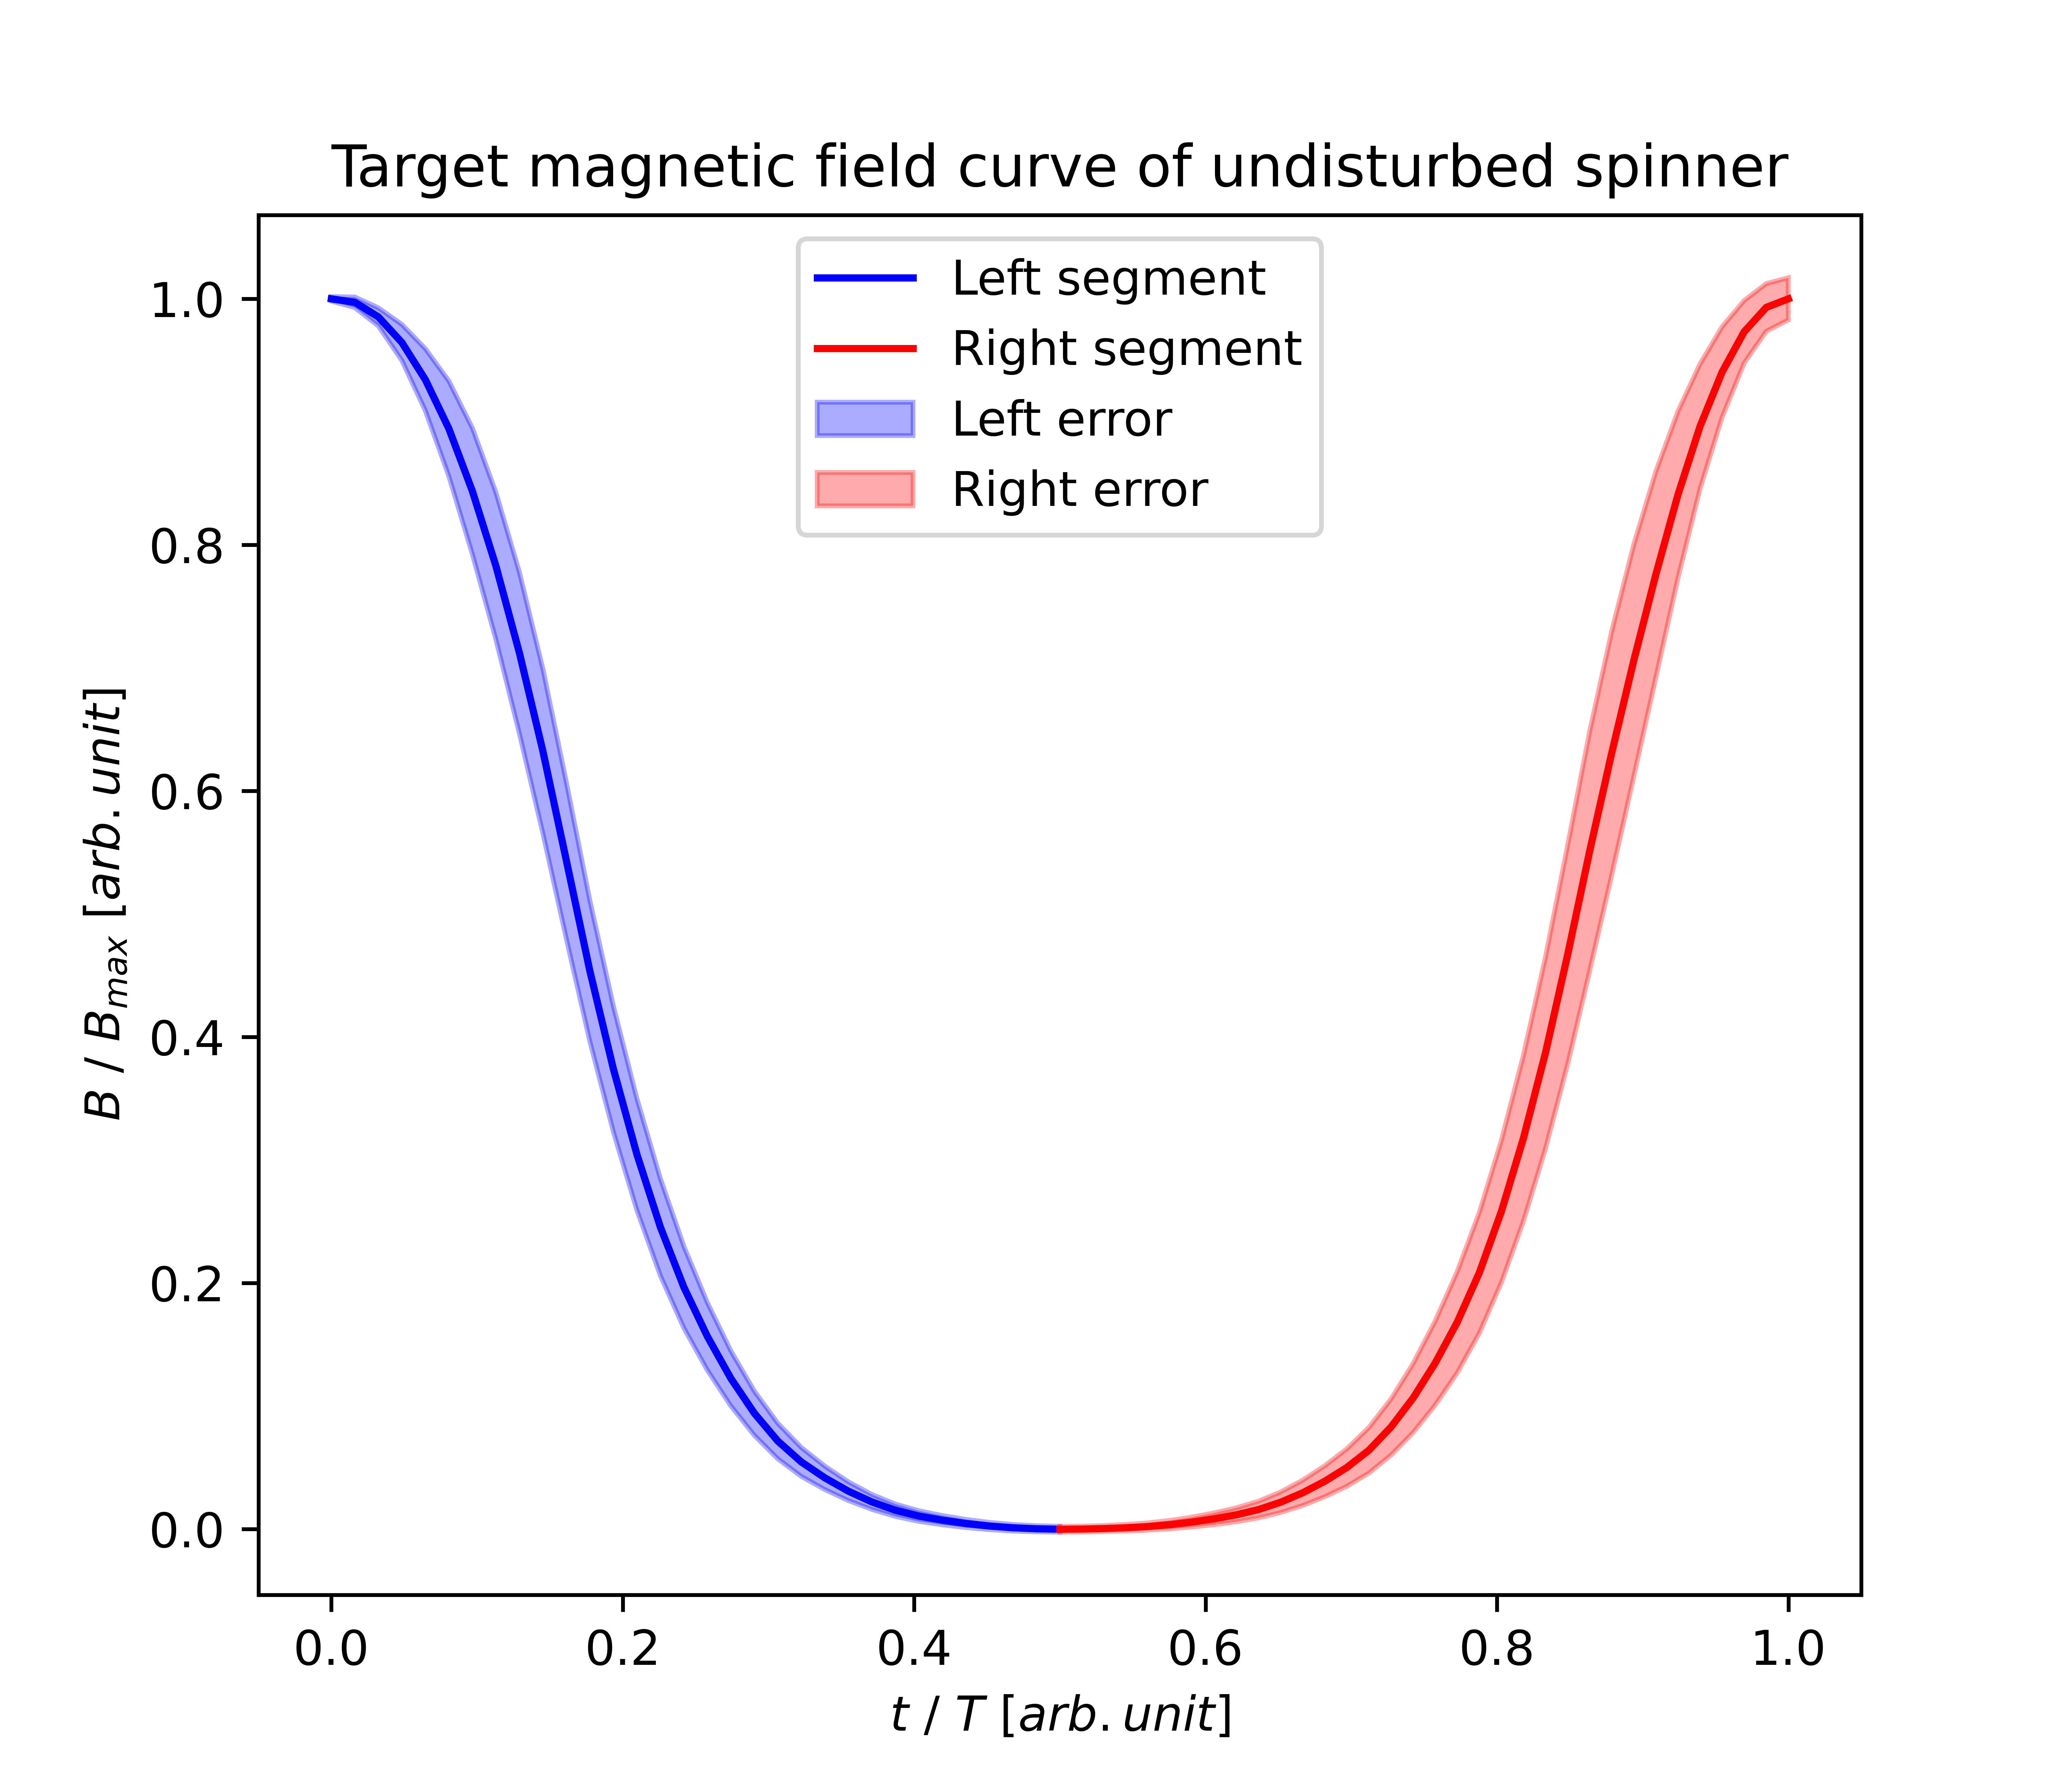
\includegraphics[width=0.5\textwidth]{target_curve.png}
    \centering
    \caption{Nerušený průběh jedné sub-periody}
    \label{fig:target_curve}
\end{wrapfigure}

Spinner osazený magnety byl tedy umístěn do vrtačky a roztáčen konstantní a známou rychlostí. Tento spinner označíme jako \textit{nerušený}, jelikož na něj nepůsobí vnější magnetické síly a je poháněn motorem, nikoliv magnetickým vázáním. Záznam z čidla je následně rozdělen podle jednotlivých peaků. Tyto úseky mezi peaky odpovídají průběhu magnetického pole v jednotlivých pootočeních spinneru od jednoho magnetu k následujícímu. Tomuto pootočení spinneru od jednoho magnetu k dalšímu (v našem případě o 120°, protože spinner má 3 ramena) budeme říkat \textit{sub-perioda}. Amplitudy a doby trvání všech sub-period jsou poté normalizovány, jelikož přesná velikost $B$ nás nezajímá, ale zajímá nás pouze tvar této křivky. Všechny sub-periody jsou následně zprůměrovány, čímž získáváme finální tvar (viz \autoref{fig:target_curve}). Tato křivka průběhu jedné sub-periody nerušeného spinneru se stane naším podkladem, vůči kterému budeme srovnávat ostatní, nyní již rušené, průběhy a vyvozovat jejich úhlové závislosti v čase. Jako poslední krok, rozdělíme cílový průběh na prosté úseky, což usnadní pozdější manipulace v algoritmu.

Všechna tři měření provedená v předchozí kapitole (viz \autoref{fig:mag_coupling_vernier}) jsou zpracována stejně jako naše kontrolní měření - rozdělena na sub-periody podle peaků, normalizována a rozdělena na prosté úseky. Nyní však nebudeme provádět průměrování, ale budeme každou sub-periodu řešit jednotlivě. Porovnání všech sub-period je k nahlédnutí v grafu \ref{fig:B_sub_periods}.

\clearpage

\begin{figure}[H]
    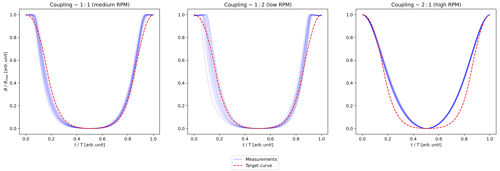
\includegraphics[width=\textwidth]{B_sub_period.png}
    \centering
    \caption[Porovnání sub-period rušených spinnerů vůči nerušenému průběhu]{Porovnání sub-period rušených spinnerů vůči nerušenému průběhu. Každá jednotlivá sub-perioda je vykreslena poloprůhlednou modrou, což umožní sledování nejčastějších průběhů, které budou tmavší.}
    \label{fig:B_sub_periods}
\end{figure}

Dalším krokem je zpětné odvození toho, jaký byl průběh úhlu v čase v těchto sub-periodách. Celá sub-perioda je rozdělena na 2 prosté úseky a tím pádem jsme v obou z nich pro náš nerušený průběh schopni přesně přiřadit, že každá naměřená hladina $B_i$ odpovídá specifickému času $t_i$, ve kterém byla naměřena, a ze znalosti rychlosti jsme ke každému času $t_i$ schopni určit přesný úhel, ve kterém se spinner v tu chvíli nacházel $\varphi_i$:

$$
    B_i \text{ } \ldots \text{ } t_i \text{ } \ldots \text{ } \varphi_i
$$

Zpětné odvození pro rušené sub-periody poté spočívá v porovnání s cílovou (nerušenou) křivkou. Pro každou naměřenou hladinu magnetického pole rušeného spinneru $B_j$ hledáme odpovídající hladiny v naší cílové křivce $B_{i1}$ a $B_{i2}$, mezi kterými se $B_j$ nachází, tedy splňuje $B_{i1} < B_j < B_{i2}$. Z jejich odpovídajících časů a úhlů pomocí lineární interpolace určíme přibližný čas, ve kterém by se $B_j$ objevilo v nerušeném případě a tedy i jaká je jeho přibližná pozice v čase $t_j$:

$$
    B_j \text{ } \ldots \text{ } t_j \text{ } \ldots \text{ } \varphi_j = \frac{B_j - B_{i1}}{B_{i2} - B_{i1}} \cdot (\varphi_{i2} - \varphi_{i1}) + \varphi_{i1}
$$

Úskalím tohoto procesu je, že když je směrnice magnetické indukce ($dB/dt = \dot{B}$) velmi malá a tedy i $B_{i2} - B_{i1}$ malé, extrémně rychle roste nepřesnost určení $\varphi_j$. Při nulové směrnici pak nejsme schopni úhel určit vůbec a chybovost je tedy nepřímo úměrná $\dot{B_i}$.

Po určení $\varphi_j$ a $t_j$ pro všechny datové body rušené sub-periody jsme schopni vytvořit závislost úhlu na čase a porovnat ji s kontrolním případem (viz \autoref{fig:ang_sub_periods}). 

\clearpage

\begin{figure}[H]
    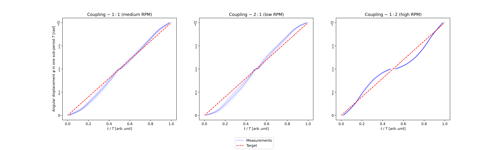
\includegraphics[width=\textwidth]{ang_sub_period.png}
    \centering
    \caption[Porovnání průběhu úhlu v sub-periodě rušených spinnerů vůči nerušenému průběhu]{Porovnání průběhu úhlu v sub-periodě rušených spinnerů vůči nerušenému průběhu. Každá sub-perioda je opět vykreslena poloprůhlednou modrou, což umožní sledování nejčastějších průběhů.}
    \label{fig:ang_sub_periods}
\end{figure}

\begin{wrapfigure}{r}{0.5\textwidth}
    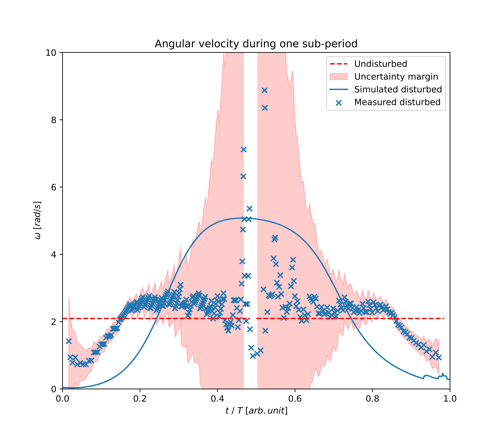
\includegraphics[width=0.5\textwidth]{ang_vel_sub_period.png}
    \centering
    \caption{Porovnání měřeného a simulovaného průběhu úhlové rychlosti v čase pro mód $2:1$}
    \label{fig:ang_vel_sub_period}
\end{wrapfigure}

Nakonec provedeme porovnání se simulací pro mód $2:1$. Porovnávat budeme úhlovou rychlost v průběhu sub-periody, kterou z měřených dat dopočítáme pomocí rozdílu vedlejších bodů. Výsledný graf lze vidět na \ref{fig:ang_vel_sub_period}. Můžeme si všimnout, že kolem středu, tedy když je $\dot{B}$ malá, je interval nepřesnosti obrovský (viz dříve zmíněné důvody).

Simulované a měřené hodnoty si jsou lehce podobné, alespoň co se tvaru křivky týče. Důvody, proč se neshodují více, mohou být mnohé. Například: nežádoucí jevy v ložisku, nepřesnost cílové křivky nebo také celková komplexita algoritmu, který pro své fungování využívá mnohé předpoklady.


\clearpage

\section{Vylepšení aparatury}

\subsection{Laserový snímač (LS)}

\begin{wrapfigure}{r}{0.45\textwidth}
    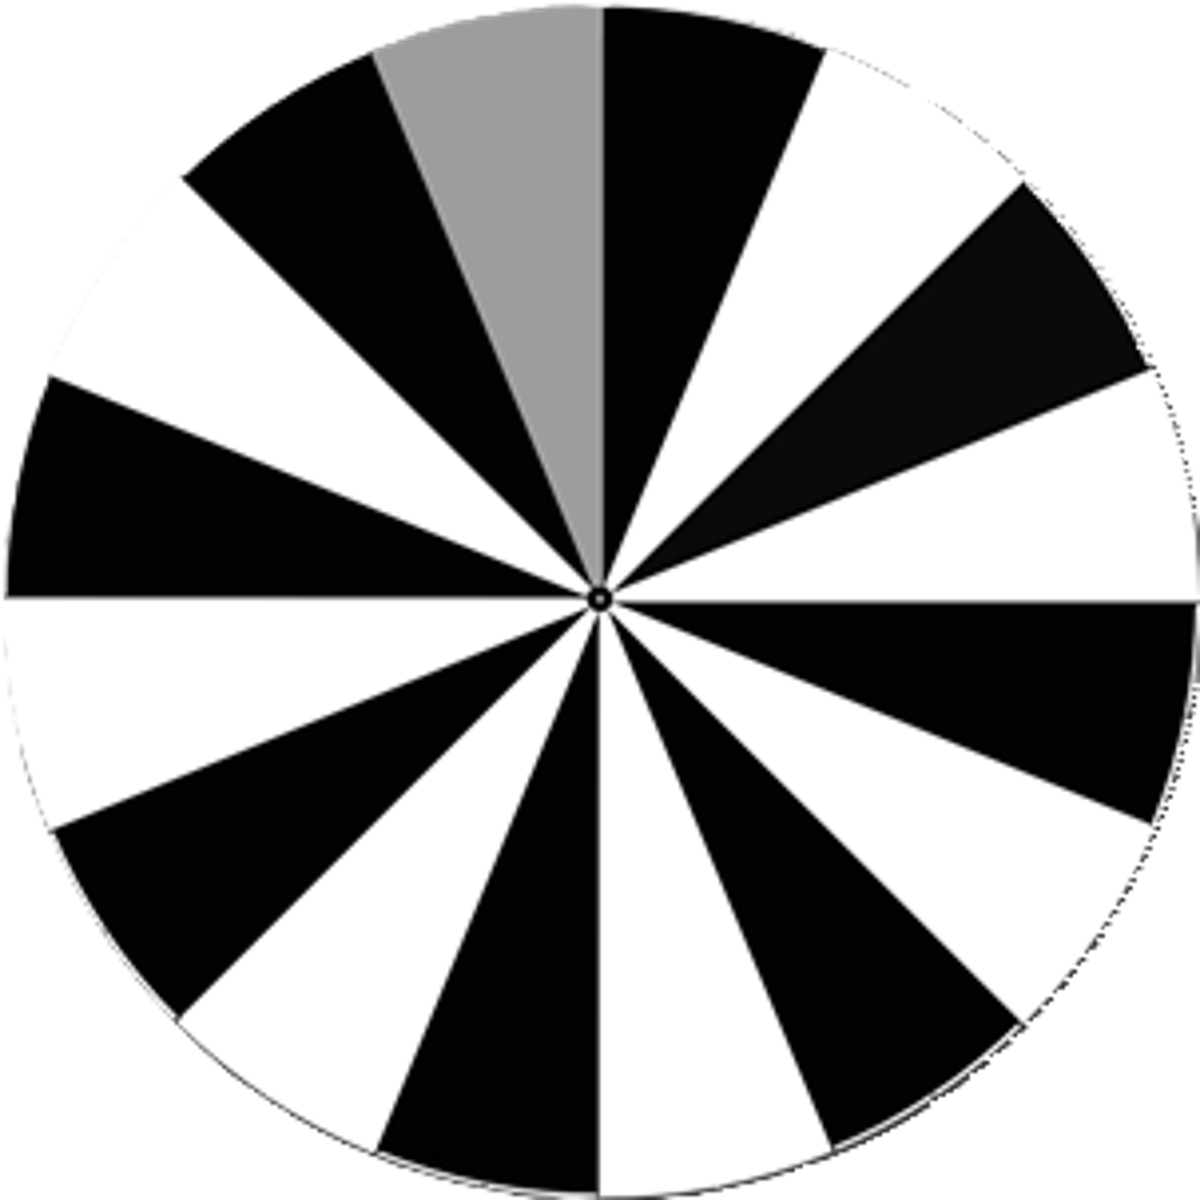
\includegraphics[width=0.30\textwidth]{laser_tracking_circle16.png}
    \centering
    \caption[Obrázek použitého absorpčního kola]{Obrázek použitého absorpčního kola (16 výsečí) na našich spinnerech. Vyšší počet výsečí je možný, ale 16 bylo pro náš případ dostačující. Šedivá výseč tvoří referenční bod, podle kterého je možné v kódu určit přesnou rotaci vůči okolí. }
    \label{fig:laser_circle16}
\end{wrapfigure}

Dříve použité metody snímání pohybu spinnerů mají své výhody i nevýhody. Nevýhodou snímání pomocí magnetického čidla je nízká přesnost a nevýhodou snímání pomocí videa je pracnost následného trackování a časová limitace záznamu.

Dalším krokem k vylepšení naší aparatury tedy bylo vytvořit lepší způsob snímání. K tomuto jsme se rozhodli vytvořit vlastní senzory postavené na principu sledování absorpce laserového paprsku fotodiodou. Na každý spinner pak byl připevněn papírový disk  se střídajícími se černými a bílými pruhy (viz \autoref{fig:laser_circle16}), které jinak absorbují světlo z laseru, čímž se mění i měřené napětí na fotodiodě. Z průběhu napětí měřeného osciloskopem jsme následně podobně schopni určit úhlovou rychlost, protože každý \\ proužek odpovídá 22.5° rotace.

\begin{wrapfigure}{r}{0.45\textwidth}
    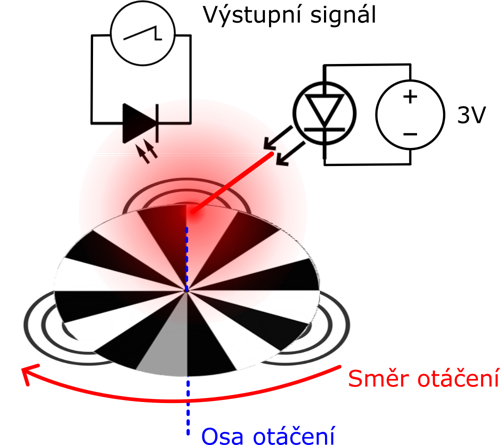
\includegraphics[width=0.45\textwidth]{laser_setup_0.png}
    \centering
    \caption{Ilustrace použití laserového snímače (LS)}
    \label{fig:LS_diode}
\end{wrapfigure}
Nyní jsou našimi limitacemi pouze vzorkovací frekvence osciloskopu, která je pro naše využití více než dostačující, a počet pruhů na papírovém kole, který můžeme dle libosti měnit.

\subsection{Zbytek aparatury}
\label{sub:main_2LS_aparature}

Celá aparatura (viz \autoref{fig:2LS_aparature}) využívá 2 laserové snímače - jeden pro hnací spinner a jeden pro hnaný spinner - a jejich výstupní signály jsou nahrávány dvoukanálovým osciloskopem. Hnací spinner je poháněn motorem, resp. vrtačkou, jejíž otáčky jsou regulovány laboratorním zdrojem napětí. Hnaný spinner je poté pevně upevněn v definované vzdálenosti od hnacího.

\clearpage
\begin{figure}[H]
    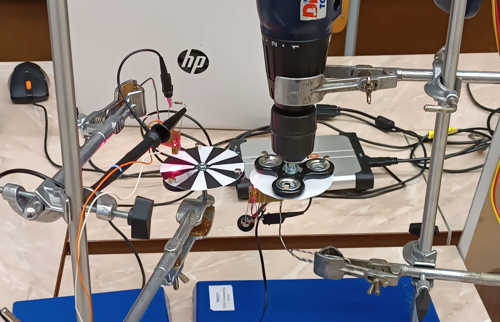
\includegraphics[width=0.7\textwidth]{2LS_aparature.png}
    \centering
    \caption{Fotografie finální aparatury}
    \label{fig:2LS_aparature}
\end{figure}
\subsection{Výsledky měření}
{
    \raggedright
    Pomocí nové, přesnější, aparatury jsme prováděli měření čtyř různých módů. U jednoho z nich jsme opakovali měření i za vyšších otáček, abychom sledovali, zda se chování vazby v tomto případě změní.
}
\begin{figure}[H]
    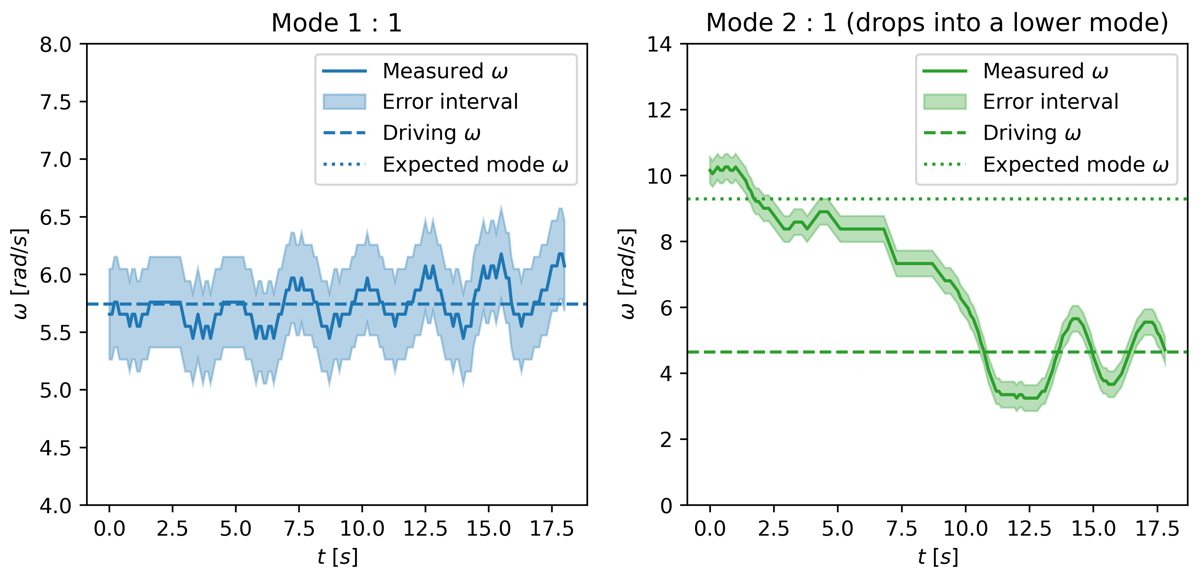
\includegraphics[width=0.8\textwidth]{magnetic_modes1.png}
    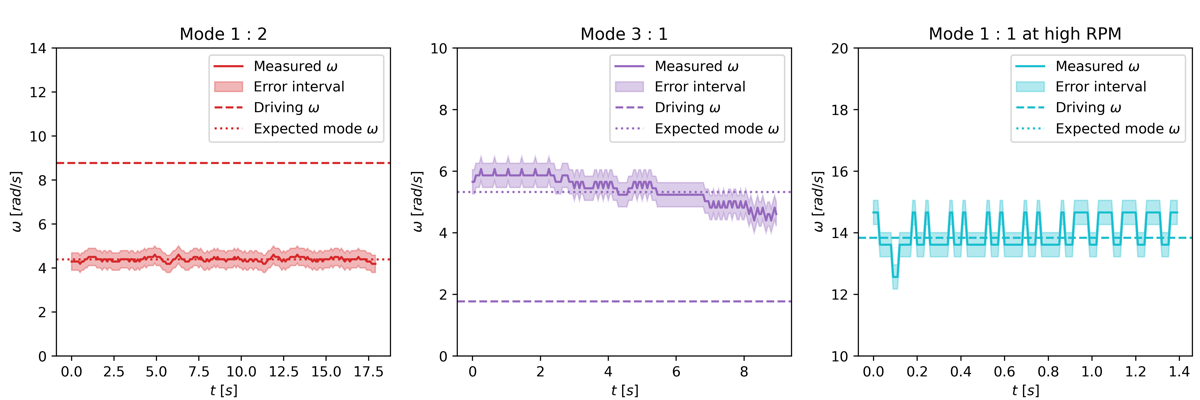
\includegraphics[width=0.8\textwidth]{magnetic_modes2.png}
    \centering
    \caption{Měření magnetické vazby pomocí LS}
    \label{fig:ang_sub_periods}
\end{figure}

Nejzajímavější pro nás jsou výsledky měření módu $1:1$ a $2:1$, jelikož na nich můžeme ukázat dva jevy objevující se v magnetické vazbě. Na měření módu $1:1$ je vidět oscilace rychlosti hnaného spinneru kolem očekávané rychlosti. K tomuto jevu dochází, protože spinnery tvořící vazbu nebyly ideálně zaklesnuty do sebe (ramena hnaného spinneru nezapadala přesně do středu mezery mezi rameny hnacího spinneru). Rameno hnaného spinneru, které nezapadá perfektně do středu mezery, je tedy blíže k jednomu z ramen hnacího spinneru, což vede k nerovnováze sil, protože z této strany na hnaný spinner působí větší síla než z druhé strany. Tento přirozený způsob vracení ramene do rovnovážné polohy se projevuje právě touto oscilací, která se objevovala již v minulém měření (viz mód $1:1$ v grafu \ref{fig:mag_coupling_vernier}).

Druhým jevem je přecházení mezi módy. Pokud je rychlostní rozdíl spinnerů příliš velký a síla vazby příliš malá, může dojít k rozbití vazby. Poté, tím že hnaný spinner ztrácí rychlost kvůli tření, může být zachycen v nižším módu, jehož interval přijatelných rychlostí je větší. K tomuto došlo v měření módu $2:1$. Spinner se chvíli držel na módu $2:1$, ale kolem šesté sekundy byla jeho rychlost kvůli tření již příliš malá a opustila interval přijatelných rychlostí pro mód $2:1$. Nyní nevázaný spinner dále zpomaloval, dokud se vazba neobnovila na nižším módu. Ihned po jejím obnovení je opět vidět oscilace kolem rovnovážné polohy, kterou jsme popisovali v předchozím odstavci. To, proč se přijatelný interval rychlostí zmenšuje, vychází z toho, že v případě módu $1:1$ zapadá do každé mezery hnacího spinneru přesně 1 rameno hnaného (resp. 1 rameno proběhne mezerou). Při módu $2:1$ "zapadají" do každé mezery dvě ramena (resp. 2 ramena musí proběhnout stejně velkou mezerou), mají tedy méně místa a přesnost fázového seřízení hraje ještě důležitější roli.

\clearpage

\section{Simulovaná vazba}

K hlubšímu pochopení magnetické vazby jsme využili dříve vytvořený simulační software. Pomocí něho můžeme sledovat chování v závislosti na více parametrech, které jsme schopni velmi definovaně určit a sledovat tak detaily chování. Námi vybranými parametry, které nejvíce ovlivňují chování, jsou:

\begin{enumerate}[topsep=0pt, partopsep=0pt]
    \setlength{\itemsep}{0pt}%
    \setlength{\parskip}{0pt}%
    \item vzálenost středů spinnerů značená $d$,
    \item počáteční poměr\footnote{Záporné znaménko uvádíme jelikož spinnery so otáčí opačným směrem.} rychlosti hnaného spinneru ku rychlosti hnacího spinneru $k_0 = -\omega_{driven} / \omega_{driving}$ ,
    \item hnací rychlost $\omega_{driving}$, která se v průběhu simulace nemění,
    \item fázový rozdíl spinnerů $\Delta \varphi$
    \item a konečně doba, po kterou simulace běží, značená $t_{run}$. 
\end{enumerate}

Změnou hodnot těchto parametrů a následným simulováním systému získáváme průběh $k(t)$ v čase. Analýzou tohoto průběhu jsme pak schopni automatizovaně klasifikovat makroskopické chování systému do několika kategorií.

K automatizovanému analyzování používáme 4 hlavní vlastnosti průběhu:
\begin{enumerate}[topsep=0pt, partopsep=0pt]
    \setlength{\itemsep}{0pt}%
    \setlength{\parskip}{0pt}%
    \item Zda $k(t)$ v průběhu celé simulace prochází nulou.
    \item Aritmetický průměr všech hodnot\footnote{$dt$ v zde určuje časový simulační krok, který byl fixovaný na $dt = 10^{-4}$s.}: $\bar{k} = \frac{dt}{t_{run}}\sum_{t=0}^{t_{run}} k(t)$.
    \item Směrnici $m$ lineárního fitu celého průběhu $k(t)$.
    \item Směrodatnou odchylku $\sigma$.
\end{enumerate}

Pomocí těchto 4 vlastností poté dělíme průběhy do 4 kategorií (viz \autoref{fig:classification_options}):

\begin{enumerate}[topsep=0pt, partopsep=0pt]
    \setlength{\itemsep}{0pt}%
    \setlength{\parskip}{0pt}%
    \item stabilní vazba (když $k(t)$ neprochází 0 a $m$ < $10^{-3}$),
    \item ustálení kolem 0 (když $k(t)$ prochází 0 a $m$ < $5\cdot10^{-5}$),
    \item slabá interakce (když $k(t)$ neprochází 0 a $m$ > $10^{-3}$),
    \item chaos (když $k(t)$ prochází 0, $m$ > $10^{-3}$ a $\sigma \gg 0.1$).
\end{enumerate}

Pro potvrzení zmenšování intervalu přijatelných rychlostí jsme nejdříve vytvořili rigorózní průzkum pro parametry $d$ a $k$ v rozmezí $7 > k > 0$ a $13$ cm $> d > 7$ cm. Zbylé parametry jsme fixovali na $\Delta \varphi = 0$, $\omega_{driving} = 10$rad/s a $t_{run} = 25$s.

Výslední klasifikační graf je k vidění na \autoref{fig:state_graph_whole}.

Detailní klasifikační graf (pro parametry v rozmezí $0.78 > k > 0.5$ a $9.3$ cm $> d > 8.4$ cm) je k vidění na \autoref{fig:state_graph_zoom}.

\begin{figure}[H]
    \includegraphics[width=0.95\textwidth]{classification_options.png}
    \centering
    \caption{Příklady různě klasifikovaných průběhů $k(t)$}
    \label{fig:classification_options}
\end{figure}

\begin{figure}[H]
    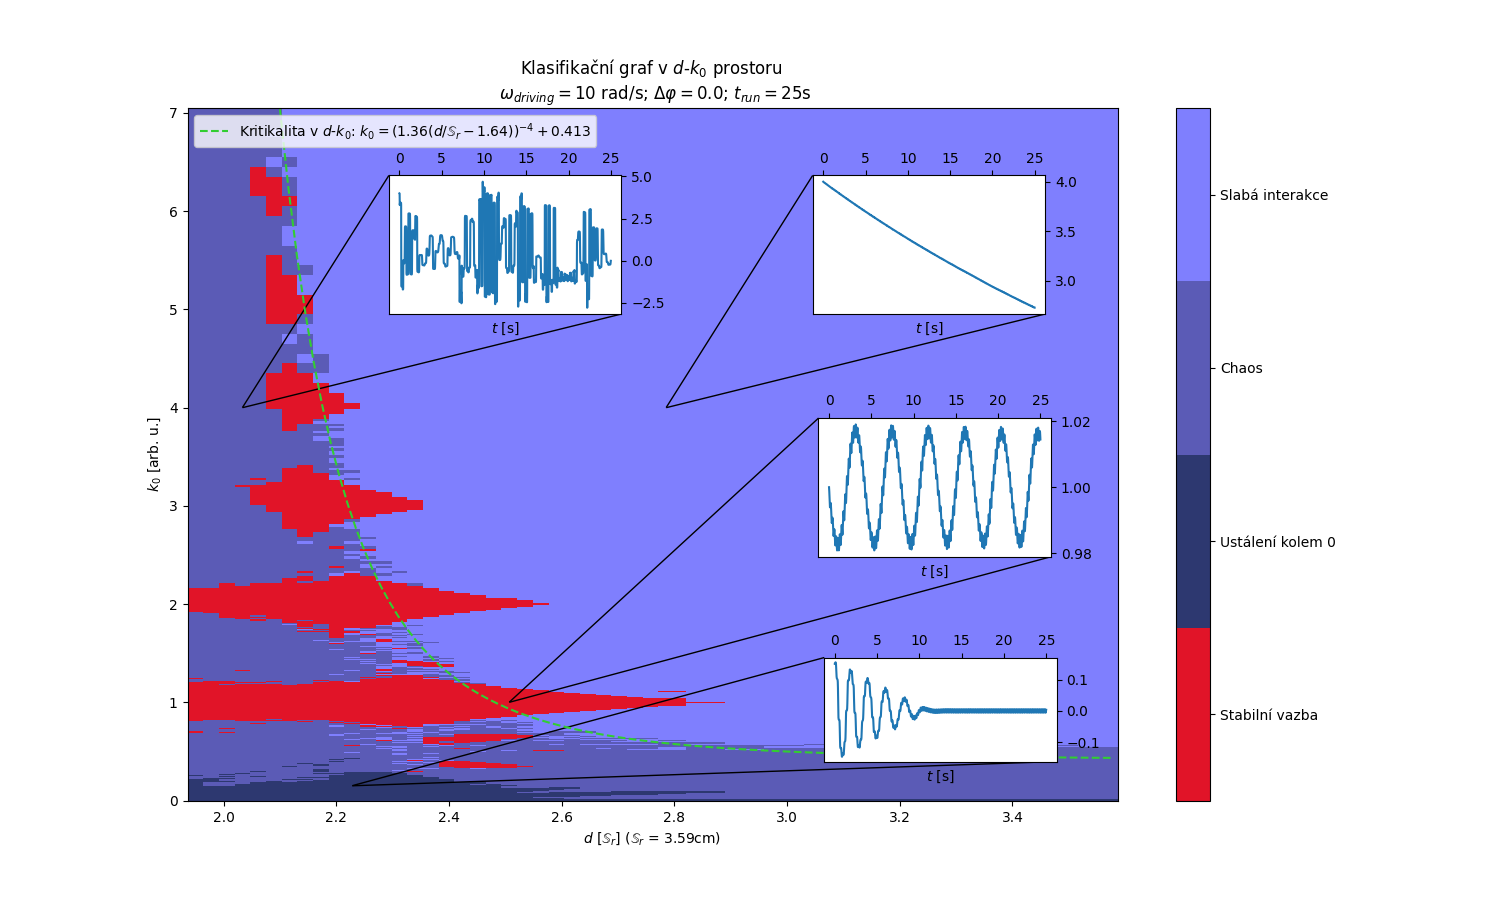
\includegraphics[width=1\textwidth]{overview_classification.png}
    \centering
    \caption{Stavový graf v závislosti na parametrech $d$ a $k_0$.}
    \label{fig:state_graph_whole}
\end{figure}

\clearpage

Tvary ostrovů stability podporují naše tvrzení, že při dané rychlosti se interval přijatelných rychlostí změnšuje s rostoucím módem. Zároveň se ale dozvídáme i to, že se tento interval zmenšuje se vzdáleností. V grafu také vidíme dva malé ostrovy pro módy 1:3, 1:2, 2:3, 4:3.

\begin{figure}[H]
    \includegraphics[width=0.49\textwidth]{overview_stable_modes.png}
    \includegraphics[width=0.49\textwidth]{overview_deviations.png}
    \centering
    \caption[Barevné oddělení ostrovů stabilních módů a směrodatná odchylka.]{Vlevo: barevně oddělené ostrovy odpovídající specifickým módům. Bílá určuje, že v tomto prostoru není stabilní mód dosažen. Vpravo: směrodatná odchylka (logaritmicky škálovaná) simulovaných systému v celé doméně. Kolem ostrovů stability sledujeme ostrou řádovou změnu.}
    \label{fig:additional_graphs_whole}
\end{figure}

\begin{figure}[H]
    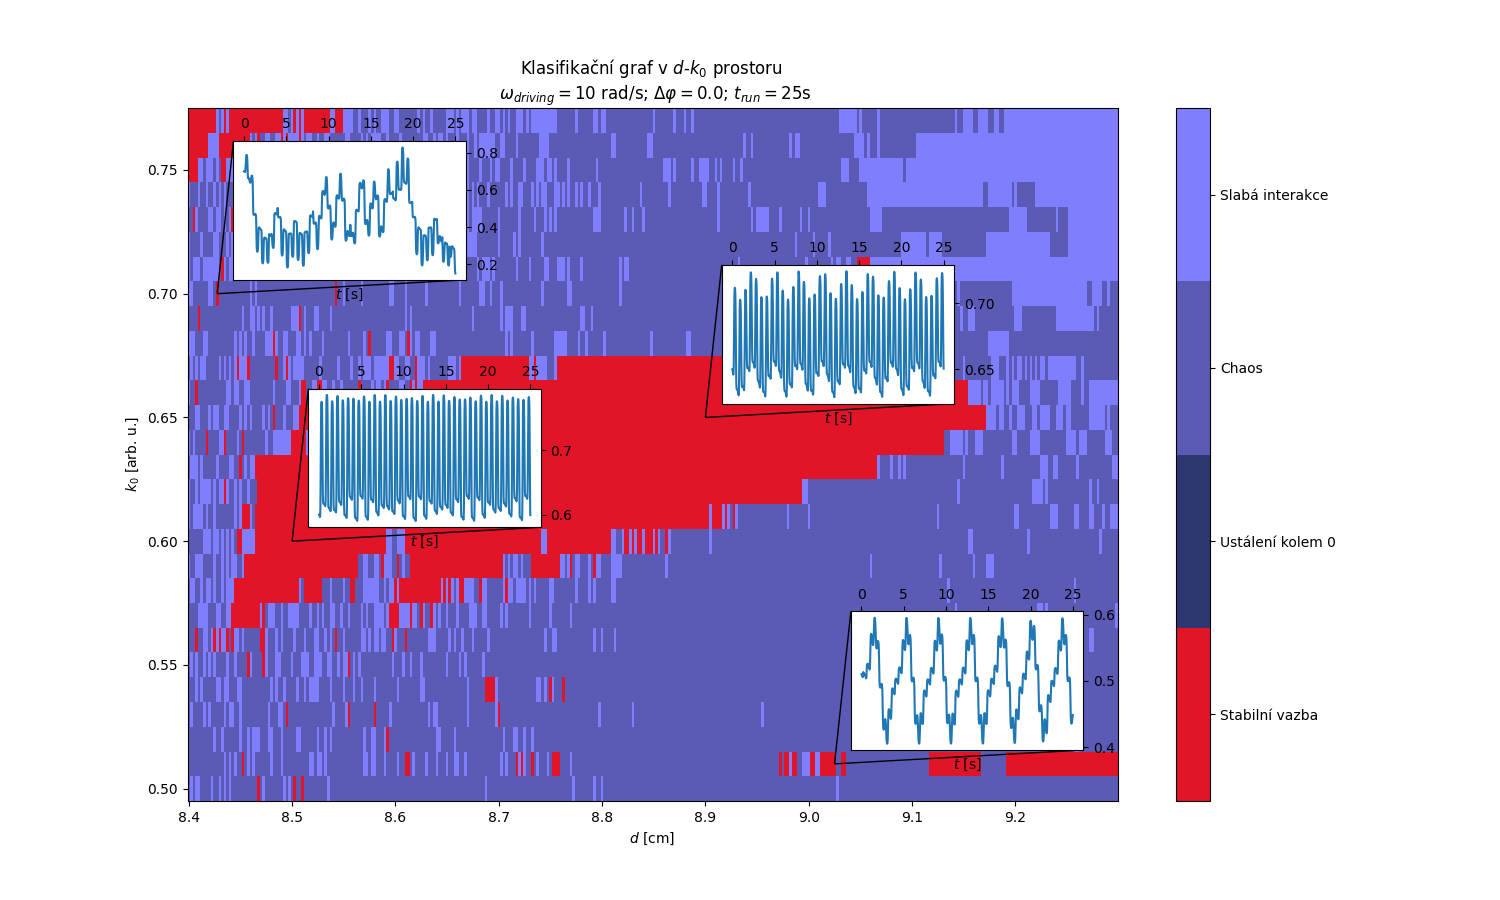
\includegraphics[width=0.49\textwidth]{zoom_classification.png}
    \includegraphics[width=0.49\textwidth]{zoom_deviations.png}
    \centering
    \caption[Detail simulovaného chování v závislosti na parametrech $d$ a $k_0$ v okolí ostrovu stability odpovídajícího módu 2:3.]{Detail simulovaného chování v závislosti na parametrech $d$ a $k_0$ v okolí ostrovu stability odpovídajícího módu 2:3. Vlevo: klasifikační graf ukazující fraktálně vypadající ostrov módu 2:3. V pravém dolním rohu je k vidění mód 1:2. Vpravo: směrodatná odchylka pro tento detail. Ostrý přechod mezi stabilitou a chaosem je opět zřejmý.}
    \label{fig:state_graph_zoom}
\end{figure}

Kromě sledování v závislosti na $d$ nás dále zajímá chování v závislosti na ostatních parametrech. Dalším parametrem, který jsme zkoumali, je $\omega_{driving}$. Následující graf \ref{fig:state_graph_omega} ukazuje chování v $\omega_{driving}$-$k_0$ prostoru:

\begin{figure}[H]
    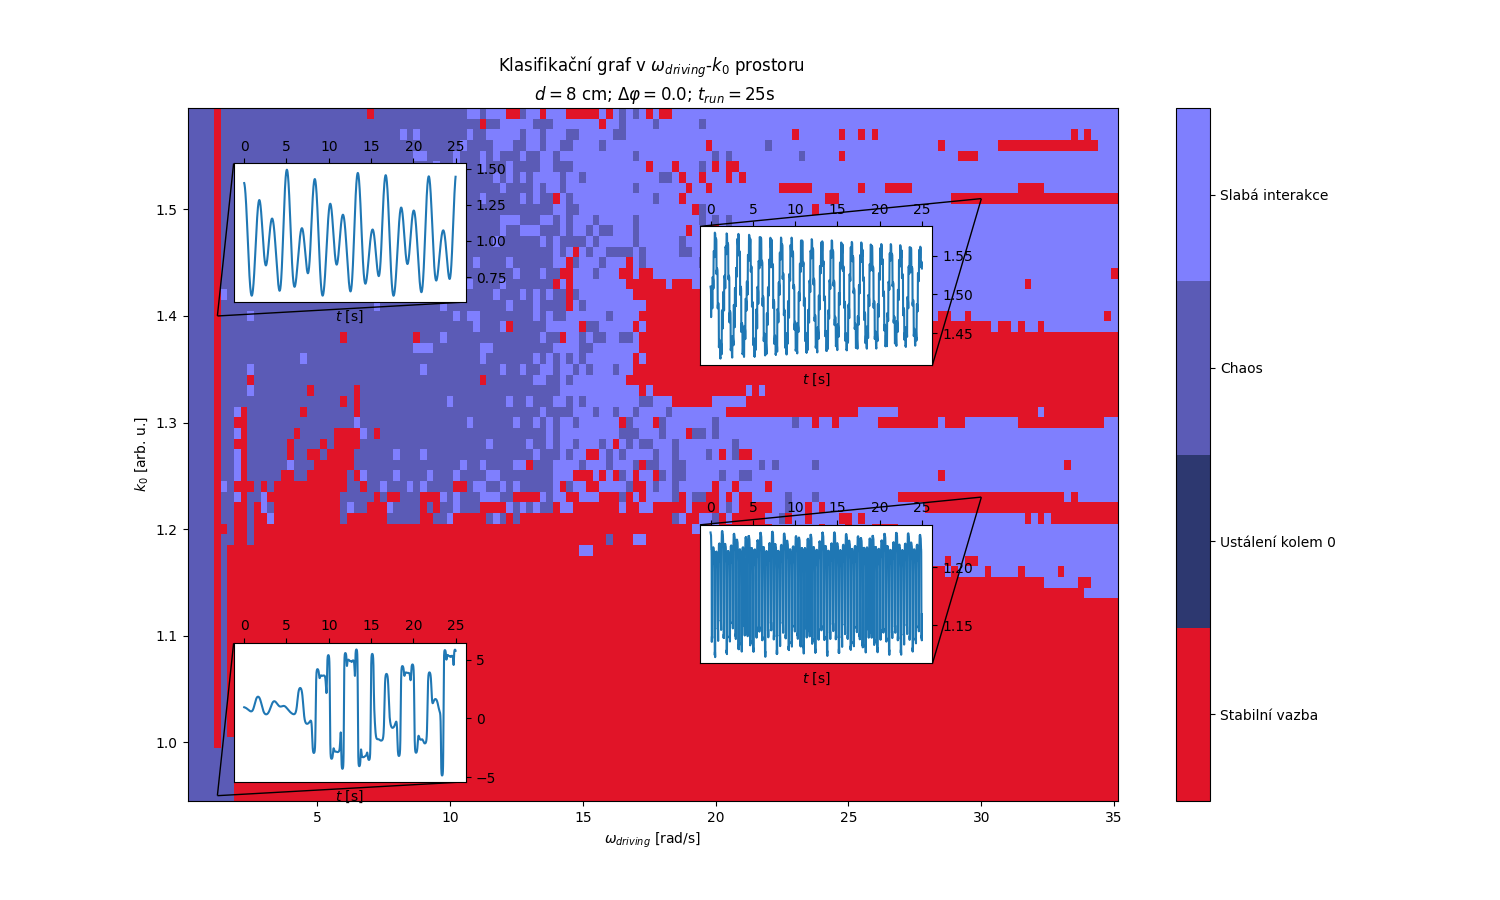
\includegraphics[width=0.49\textwidth]{omega_classification.png}
    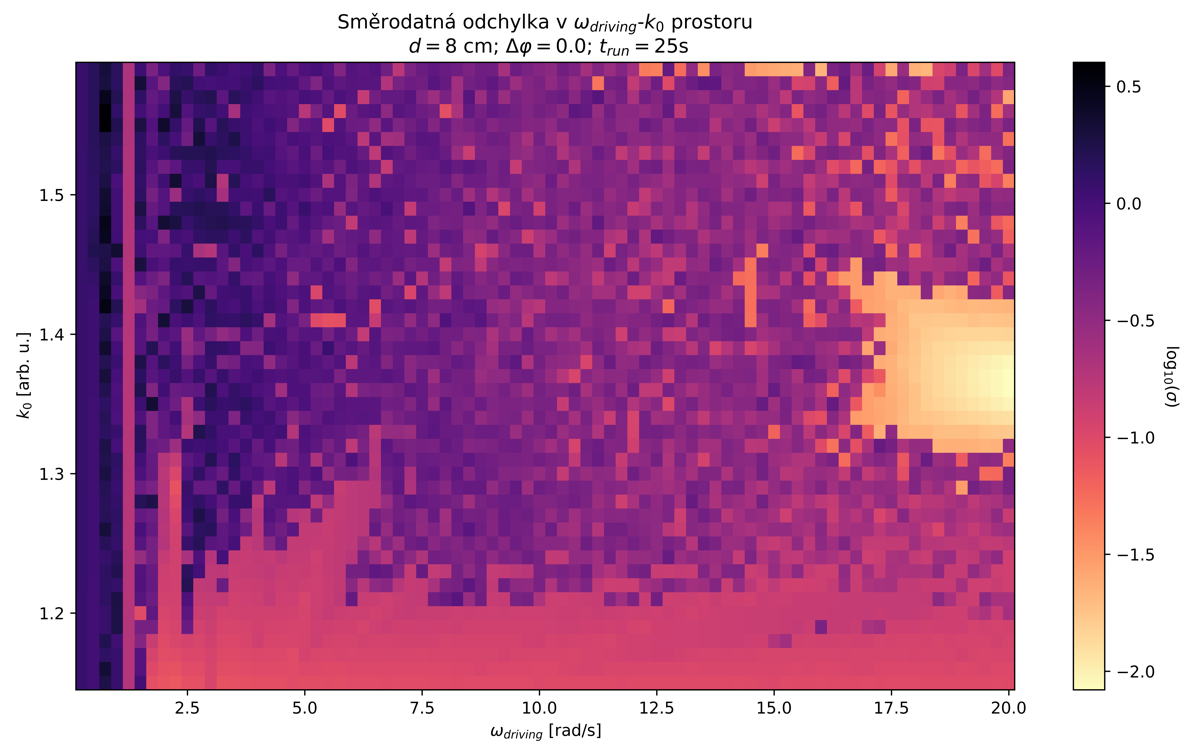
\includegraphics[width=0.49\textwidth]{omega_deviations.png}
    \centering
    \caption[Detail simulovaného chování v závislosti na parametrech $\omega_{driving}$ a $k_0$ v okolí ostrovu stability odpovídajícího módu 4:3.]{Detail simulovaného chování v závislosti na parametrech $\omega_{driving}$ a $k_0$ v okolí ostrovu stability odpovídajícího módu 4:3. Vlevo: klasifikační graf. Vpravo: směrodatná odchylka ukazující vysokou stabilitu módu 4:3 při vysokých otáčkách.}
    \label{fig:state_graph_omega}
\end{figure}

Zajímavou oblastí v tomto grafu se stává okolí bodu $\omega_{driving} = 19$ rad/s; $k_0=1.35$, protože v této oblasti se objevuje nový mód, 4:3, který nám z dřívějších experimentů nebyl známý.